\section{Конструкторский раздел}

\subsection{Последовательность преобразований}

Последовательность выполняемых действий в ПО в виде IDEF0 представлена на рисунках \ref{idef1} и \ref{idef2}.

\begin{figure}[H]
	\centering{
		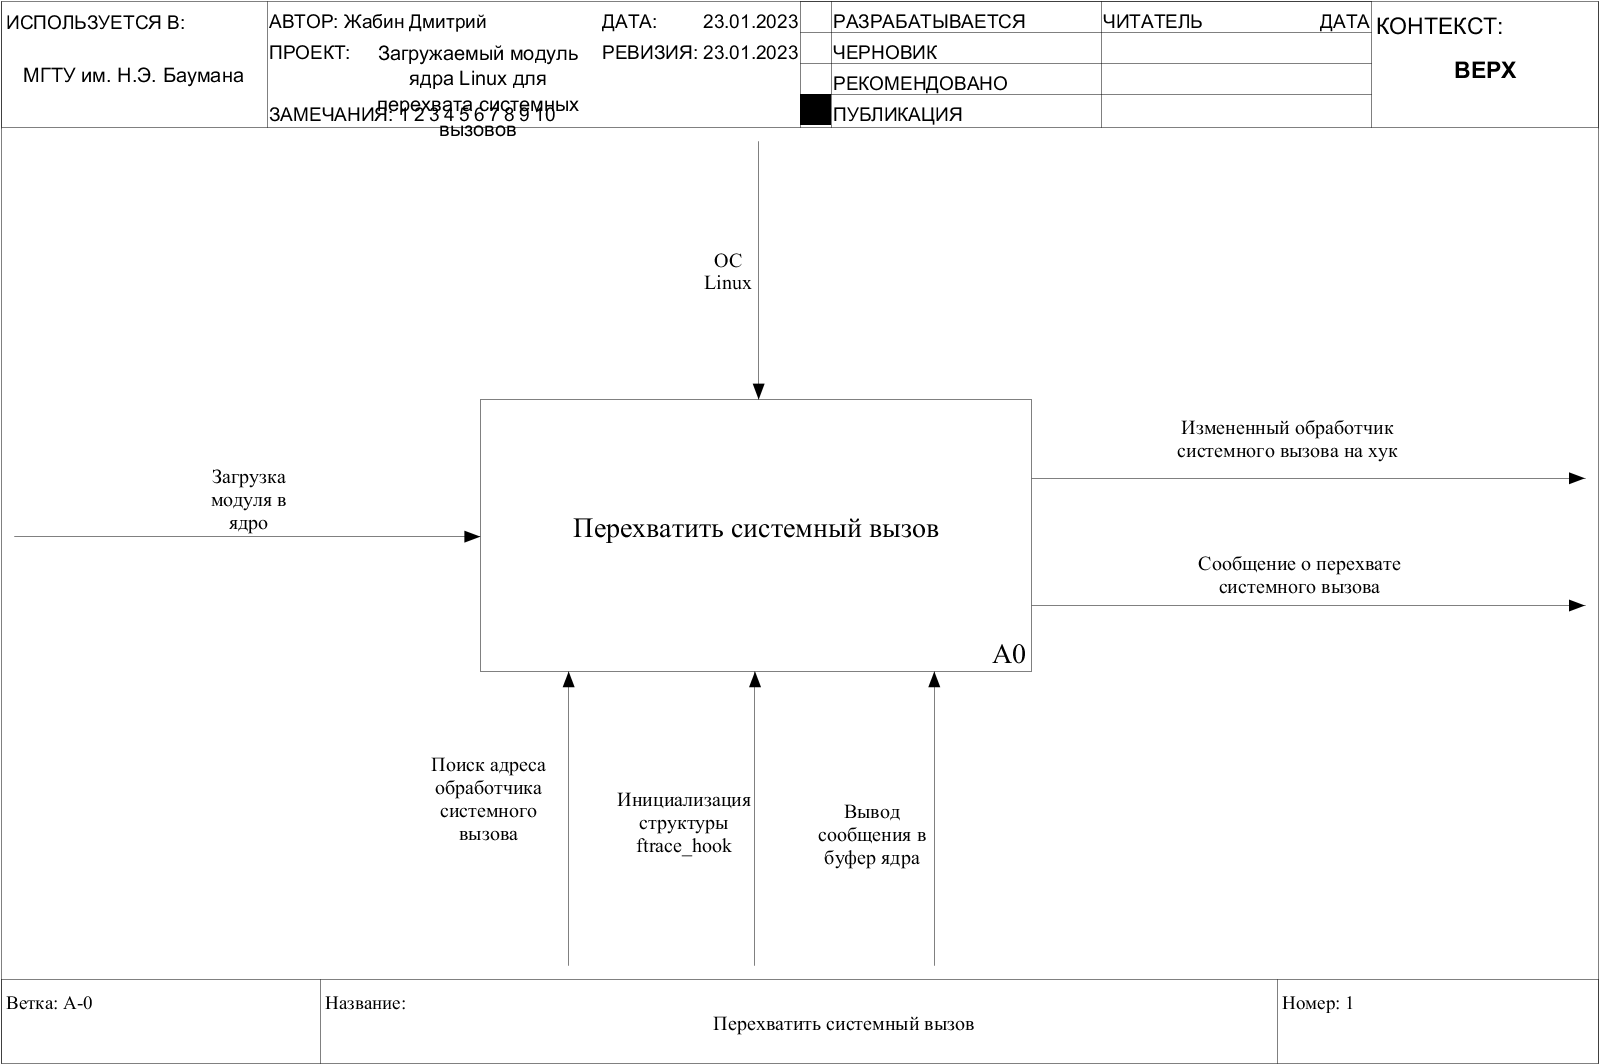
\includegraphics[width=1\textwidth]{img/idef1.png}
		\caption{Последовательность преобразований. Часть 1}
		\label{idef1}}
\end{figure}

\begin{figure}[H]
	\centering{
		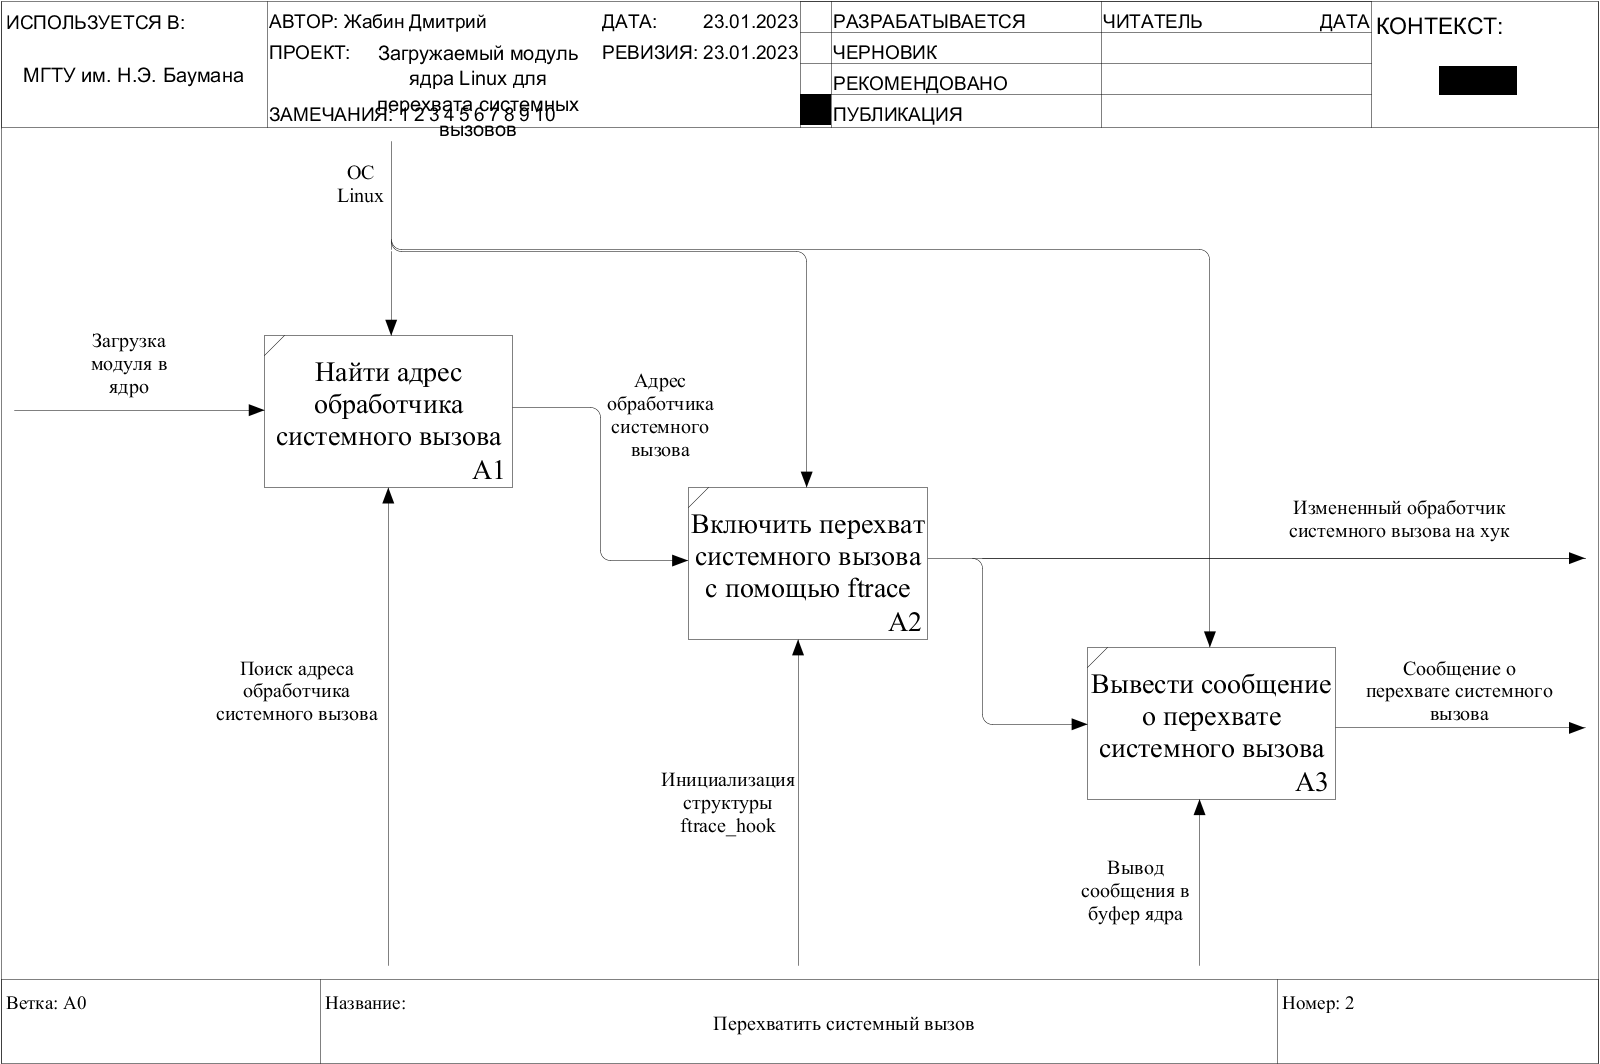
\includegraphics[width=1\textwidth]{img/idef2.png}
		\caption{Последовательность преобразований. Часть 2}
		\label{idef2}}
\end{figure}

\pagebreak

\subsection{Перехват системного вызова}

Схема алгоритма перехвата системного вызова показана на рисунке \ref{hook}.

\begin{figure}[H]
	\centering{
		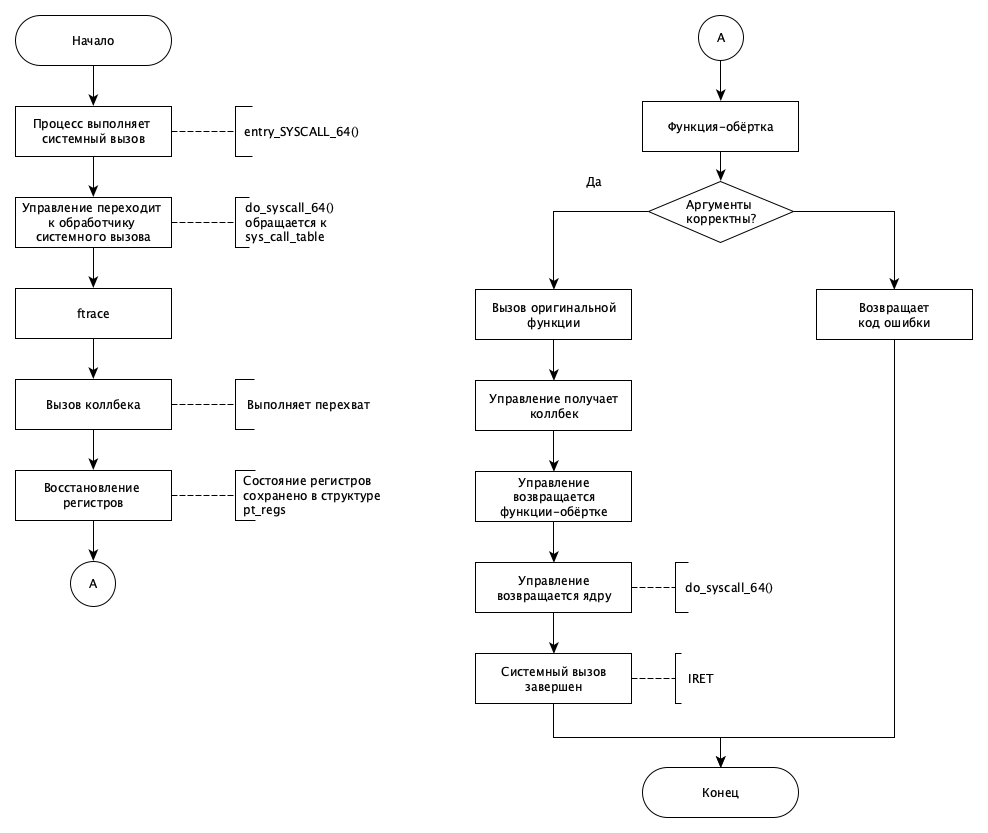
\includegraphics[width=1\textwidth]{img/alg.png}
		\caption{Алгоритм перехвата системного вызова}
		\label{hook}}
\end{figure}

\textbf{Алгоритм перехвата системного вызова}

1. Пользовательский процесс выполняет SYSCALL. С помощью этой инструкции выполняется переход в режим ядра и управление передается низкоуровневому обработчику системных вызовов — entry\_SYSCALL\_64(). Он отвечает за все системные вызовы 64-битных программ на 64-битных ядрах.

2. Управление переходит к конкретному обработчику. Ядро передает управление высокоуровневой функции do\_syscall\_64(). Эта функция в свою очередь обращается к таблице обработчиков системных вызовов sys\_call\_table и вызывает конкретный обработчик по номеру системного вызова -- sys\_execve().

3. Вызывается ftrace. В начале каждой функции ядра находится вызов функции \_\_fentry\_\_(), которая реализуется фреймворком ftrace.

4. Ftrace вызывает разработанный коллбек.

5. Коллбек выполняет перехват.

6. Ftrace восстанавливает регистры. Следуя флагу FTRACE\_SAVE\_REGS, ftrace сохраняет состояние регистров в структуре pt\_regs перед вызовом обработчиков. При завершении обработки ftrace восстанавливает регистры из этой структуры. Коллбек изменяет регистр IP, что в итоге приводит к передаче управления по новому адресу.

7. Управление получает хук. Вместо sys\_execve() управление получает функция hook\_sys\_execve(). При этом остальное состояние процессора и памяти остается без изменений, поэтому хук получает все аргументы обработчика и при завершении вернет управление в функцию do\_syscall\_64().

8. Функция hook\_sys\_execve() вызывает обработчик системного вызова. Она может проанализировать аргументы и контекст системного вызова и запретить или разрешить процессу его выполнение. В случае запрета функция возвращает код ошибки. Иначе же ей следует вызвать обработчик -- sys\_execve() вызывается повторно через указатель orig\_sys\_execve, который был сохранен при настройке перехвата.

9. Управление получает коллбек. Как и при первом вызове sys\_execve(), управление опять проходит через ftrace и передается в коллбек.
 
10. Коллбек ничего не делает, потому что в этот раз функция sys\_execve() вызывается функцией hook\_sys\_execve(), а не ядром из do\_syscall\_64(). Поэтому коллбек не модифицирует регистры и выполнение функции sys\_execve() продолжается как обычно.
 
11. Управление возвращается хуку.

12. Управление возвращается ядру. Функция hook\_sys\_execve() завершается и управление переходит в do\_syscall\_64(), которая считает, что системный вызов был корректно завершен.

13. Управление возвращается в пользовательский процесс. Ядро выполняет инструкцию IRET, системный вызов завершен.

\subsection{Алгоритм включения перехвата}

Ftrace позволяет трассировать функции, но предварительно необходимо найти адрес перехватываемой функции, чтобы вызывать ее.
Также нужно определить коллбек, который ftrace будет вызывать при трассировке функции. В коллбеке нужно заменить значение регистра IP на адрес нового обработчика, таким образом хук перехватит управление.
Для включения перехвата необходимо сначала включить ftrace для перехватываемой функции, а затем разрешить ftrace вызывать коллбек.

Схема алгоритма включения перехвата системного вызова приведена на рисунке \ref{insthook}.

\begin{figure}[H]
	\centering{
		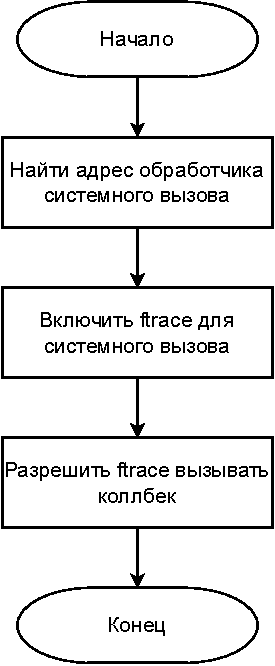
\includegraphics[width=0.3\textwidth]{img/install_hook.pdf}
		\caption{Алгоритм включения перехвата}
		\label{insthook}}
\end{figure}

\subsection{Алгоритм отключения перехвата}

Для отключения перехвата функции необходимо выполнить обратные действия: запретить ftrace вызывать коллбек, а затем отключить ftrace для системного вызова.

Схема алгоритма отключения перехвата системного вызова приведена на рисунке \ref{remhook}.

\begin{figure}[H]
	\centering{
		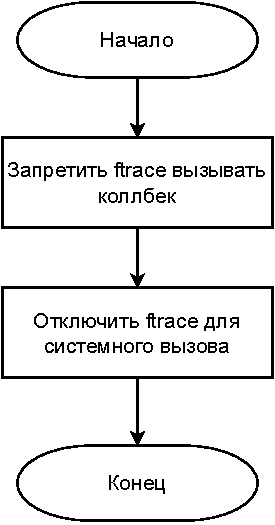
\includegraphics[width=0.3\textwidth]{img/remove_hook.pdf}
		\caption{Алгоритм отключения перехвата}
		\label{remhook}}
\end{figure}

\subsection{Структура ПО}

В состав программного обеспечения входит один загружаемый модуль ядра, который обеспечивает перехват системных вызовов, с последующим сбором информации и ее визуализацией.

\pagebreak

Структура разрабатываемого программного обеспечения представлена на рисунке \ref{structure}.

\begin{figure}[H]
	\centering{
		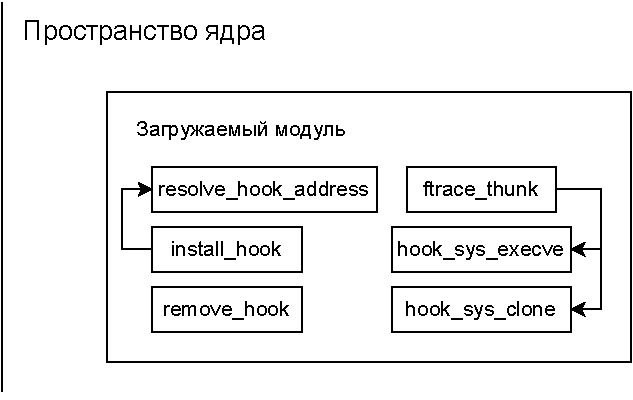
\includegraphics[width=0.7\textwidth]{img/structure.pdf}
		\caption{Структура ПО}
		\label{structure}}
\end{figure}

\subsection{Настройка средств визуализации лог-файлов}

Собранные данные о вызове функций хранятся в лог-файле /var/log/syslog. Для того, чтобы передать их в платформу Grafana для визуализации, необходимо настроить Promtail для считывания данных из лог-файла и их дальнейшей передачи в Loki для хранения.

Фрагмент конфигурационного файла Promtail представлен в листинге \ref{promt}.

\lstinputlisting[
language=C,
firstline=11,
lastline=18,
caption={Конфигурационный файл Promtail},
label={promt},
style=customc
]
{listings/promt.yaml}

\pagebreak

Собранные данные Loki отправляет на порт 3100. Настройка Grafana для прослушивания Loki на этом порту представлена на рисунке \ref{grafset}.

\begin{figure}[H]
	\centering{
		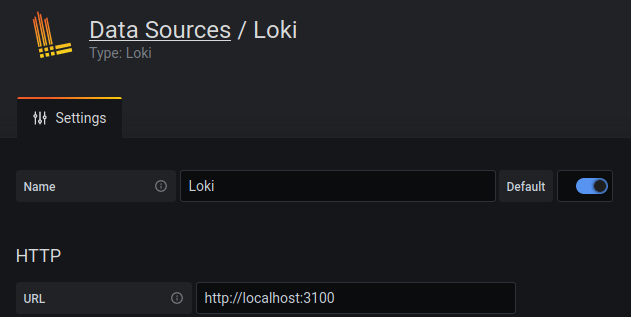
\includegraphics[width=1\textwidth]{img/grafset.png}
		\caption{Настройка Grafana}
		\label{grafset}}
\end{figure}

\pagebreak